\begin{abstract}
  The singular value spectrum of a data matrix is commonly used to detect high-dimensional
  signals.  However, as the size of this data matrix grows, taking its SVD becomes
  intractable. We consider projecting the data matrix into a lower dimensional space and
  using the resulting singular value spectrum for signal detection. We derive the almost
  sure limit of the top singular values of the resulting projected matrix both when using
  a Gaussian and unitary projection matrix. We highlight our prediction accuracy and
  discuss the benefits and drawbacks of each projection matrix using numerical simulations.
\end{abstract}
\section{Introduction}

In many classical signal processing applications, we stack observations in a data matrix
that is assumed low-rank plus noise, modeled as
\beq\label{eq:chpt7:data_model}
\widetilde{X}_n= \sum_{i=1}^r\theta_i u_iv_i^T + X_n.
\eeq
In the above equation, for $i=1,\dots,r$, $u_i\in\complex^{n\times 1}$ and
$v_i\in\complex^{N\times 1}$ are independent unit norm signal vectors, $\theta_i>0$ are
the associated signal values and $X_n$ is a noise-only matrix. Assume that
$u_i^Hu_j=\delta_{\left\{i=j\right\}}$ and $v_i^Hv_j = \delta_{\left\{i=j\right\}}$. Let
$X_n\in\complex^{n\times N}$ be a real or complex random matrix. Let 
$\sigma_1,\dots,\sigma_{\min(n,N)}$ be the singular values of $X_n$. Let $\mu_{X_n}$ be the
empirical singular value distribution, i.e, the probability measure defined as
\be
\mu_{X_n}(x) = \frac{1}{\min(n,N)}\sum_{i=1}^{\min(n,N)}\delta_{\sigma_i}(x).
\ee

In many signal processing applications, we treat the columns of $\widetilde{X}_n$ as noisy
observations of a desired target signal lying in the span of
$\left\{u_1,\dots,u_r\right\}$. In this light, we treat $\theta_i$ as the signal-to-noise
ratio (SNR) for its corresponding subspace component, $n$ as the intrinsic dimension of
the problem, and $N$ as the number of samples (or snapshots or observations) we have at our
disposal. To recover the underlying signal subspace, $\Span\left\{u_1,\dots,u_r\right\}$,
it is common to take the left singular vectors of $\widetilde{X}_n$ corresponding to the
largest $r$ singular values. The accuracy of this estimate is well studied (see
\cite{paul2007asymptotics,benaych2011eigenvalues,asendorf2013performance,benaych2012singular}).
Specifically, when $X_n$ has independent $\mathcal{CN}(0,1)$ entries, the
individual subspace component estimates are known to have a non-random estimate when
$\theta_i>\left(\frac{n}{N}\right)^{1/4}$.

However, in many such applications the intrinsic dimension, $n$, of the system is so large
that taking the SVD of $\widetilde{X}_n$ may not be tractable. In this paper, we explore the
performance of signal detection when randomly projecting $\widetilde{X}$ into a lower
dimensional space using either a Gaussian or unitary projection. Specifically for $m<n$, let
$G_n\in\complex^{n\times m}$ be a random matrix with independent $\mathcal{CN}(0,1)$
entries and let $Q_n\in\complex^{n\times m}$ be a unitary matrix such that $Q_n^HQ_n=
I_m$. Define the $m\times N$ complex matrices
\beq\label{eq:chpt7:yn}
Y_n^G = G_n^H\widetilde{X}_n,\,\,\,\,Y_n^Q = Q_n^H\widetilde{X}_n
\eeq

Since $m<n$, taking the SVD of $Y_n^G$ and $Y_n^Q$ is more tractable than taking the SVD
of $\widetilde{X}_n$. Such compressed sensing strategies for both unitary
\cite{belabbas2007fast,gu1996efficient,rudelson2007sampling} and Gaussian
\cite{hehyperspectral,rokhlin2009randomized,halko2011algorithm} sensing matrices have been
extensively studied. These algorithms have been extended to include Gaussian-like
strategies that employ matrices with partially observed entries
\cite{achlioptas2007fast,arora2006fast} as well as unitary-like strategies that use a
discrete Fourier transform matrix \cite{liberty2007randomized} or discrete cosine transform
\cite{ramachandra2011compressive}. For excellent reviews of such compressed sensing
algorithms please see \cite{halko2011finding,candes2006near,donoho2006compressed}, for
example. 

These works examine the ability of such matrices to approximate the original data matrix
as low rank. In this paper, we consider the fundamental limits of the resulting singular
values when used to detect low-rank signals. We quantify how the dimensions of our
matrices, $m,n,N$, and the SNR $\theta$ affect the behavior of the largest singular values
of $Y_n^G$ and $Y_n^Q$. Finally, we compare the detection performance of these two
specific choices of the projection matrix and show that a unitary projection matrix can
more reliably detect low-rank signals than a Gaussian projection matrix.

This paper is organized as follows. In Section \ref{sec:chpt7:main_results}, we provide
the main results of this paper including the almost sure limit of the top singular values
of the projection matrices in (\ref{eq:chpt7:yn}). We then provide corollaries to the main
result that highlight a phase transition below which signal detection is impossible and a
closed form expression of our main theorem for unitary projections. In Section
\ref{sec:chpt7:emp_res}, we verify our asymptotic results on finite sized systems and
highlight the accuracy of our predictions. We provide concluding remarks in Section
\ref{sec:chpt7:concl}.

\begin{comment}
\begin{figure*}
\begin{center}
  \subfigure[$\widetilde{X}$]{
    \label{fig:chpt7:motiv_full1}
    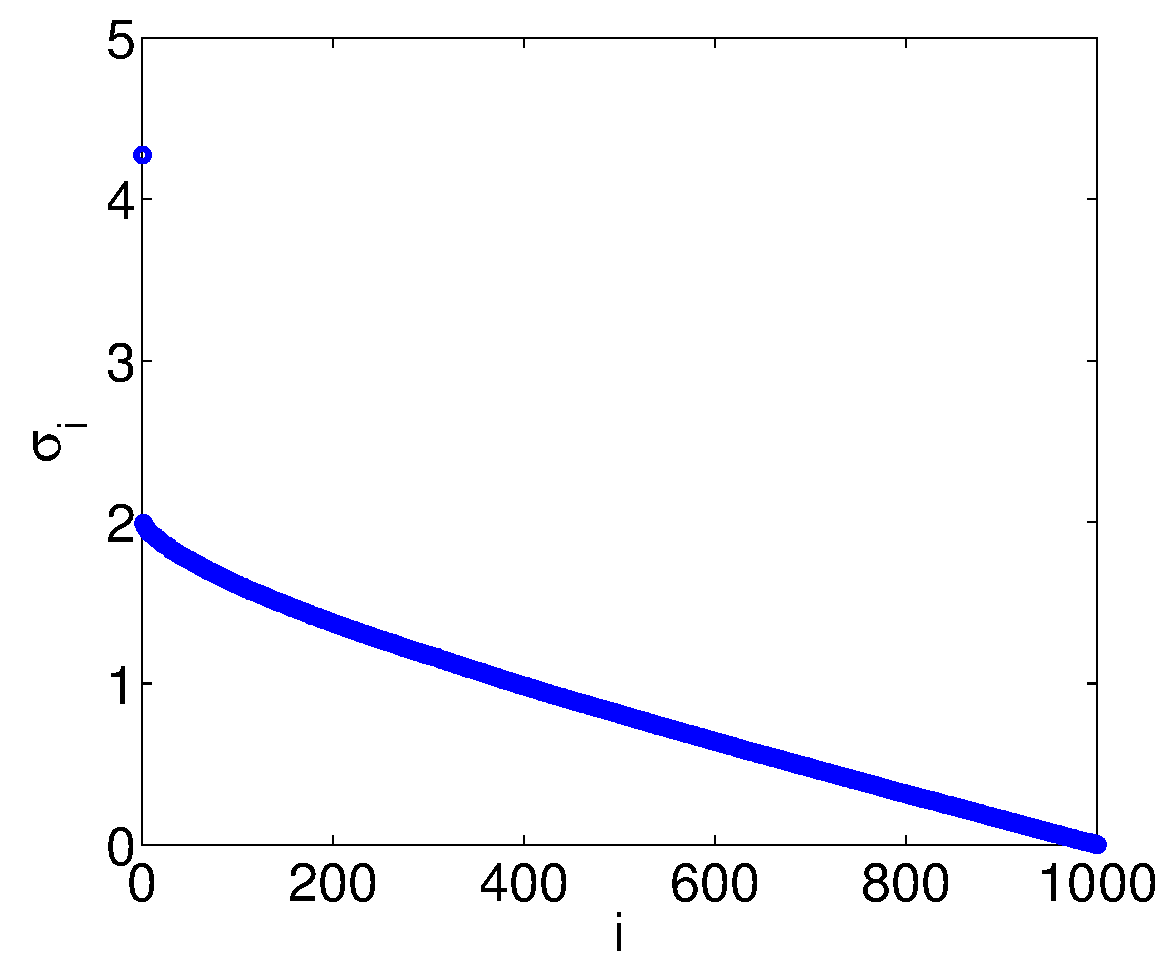
\includegraphics[width=0.3\textwidth]{chpt7_svd_proj/figs/motiv_full_1.pdf}
  }
  \subfigure[$Q^H\widetilde{X}$]{
    \label{fig:chpt7:motiv_orth1}
    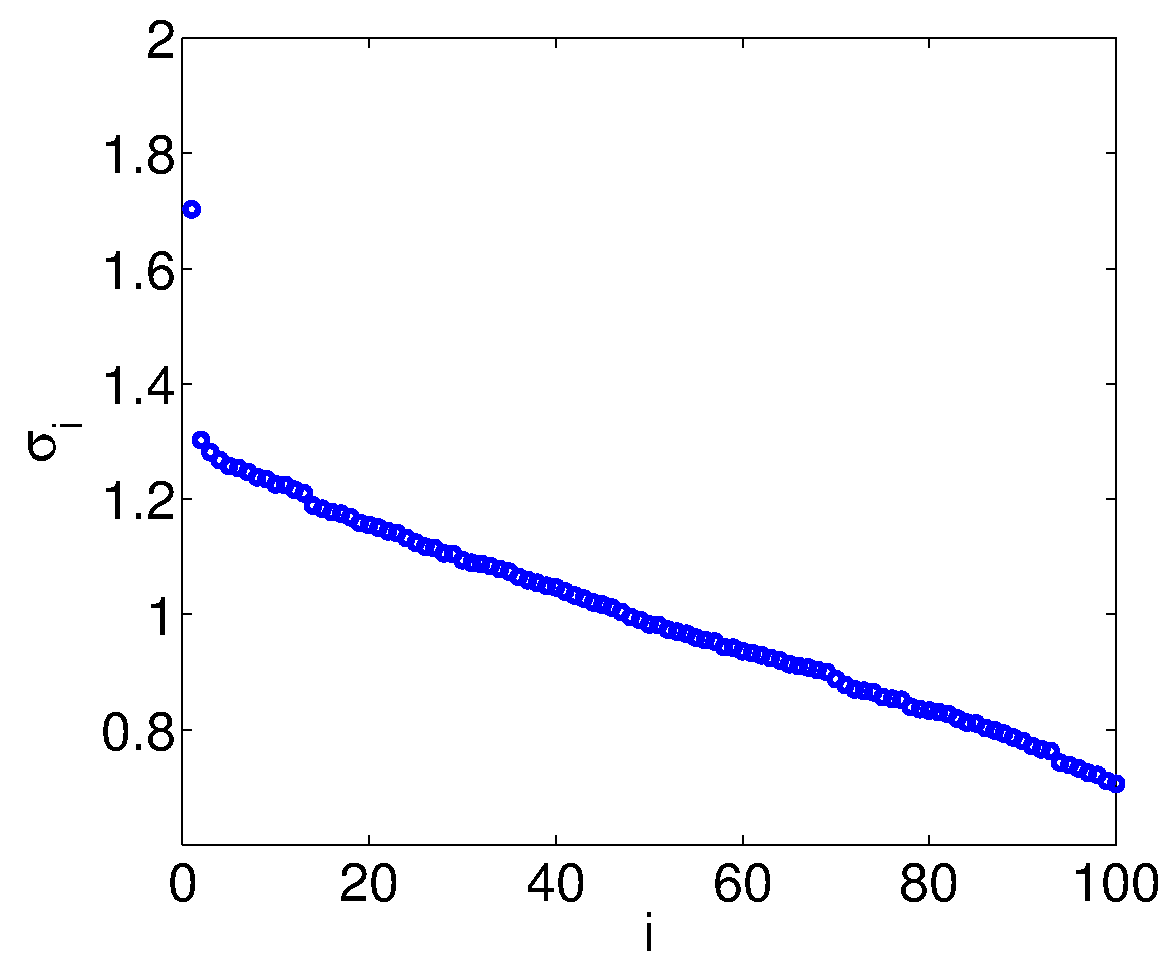
\includegraphics[width=0.3\textwidth]{chpt7_svd_proj/figs/motiv_orth_1.pdf}
  }
  \subfigure[$G^H\widetilde{X}$]{
    \label{fig:chpt7:motiv_gauss1}
   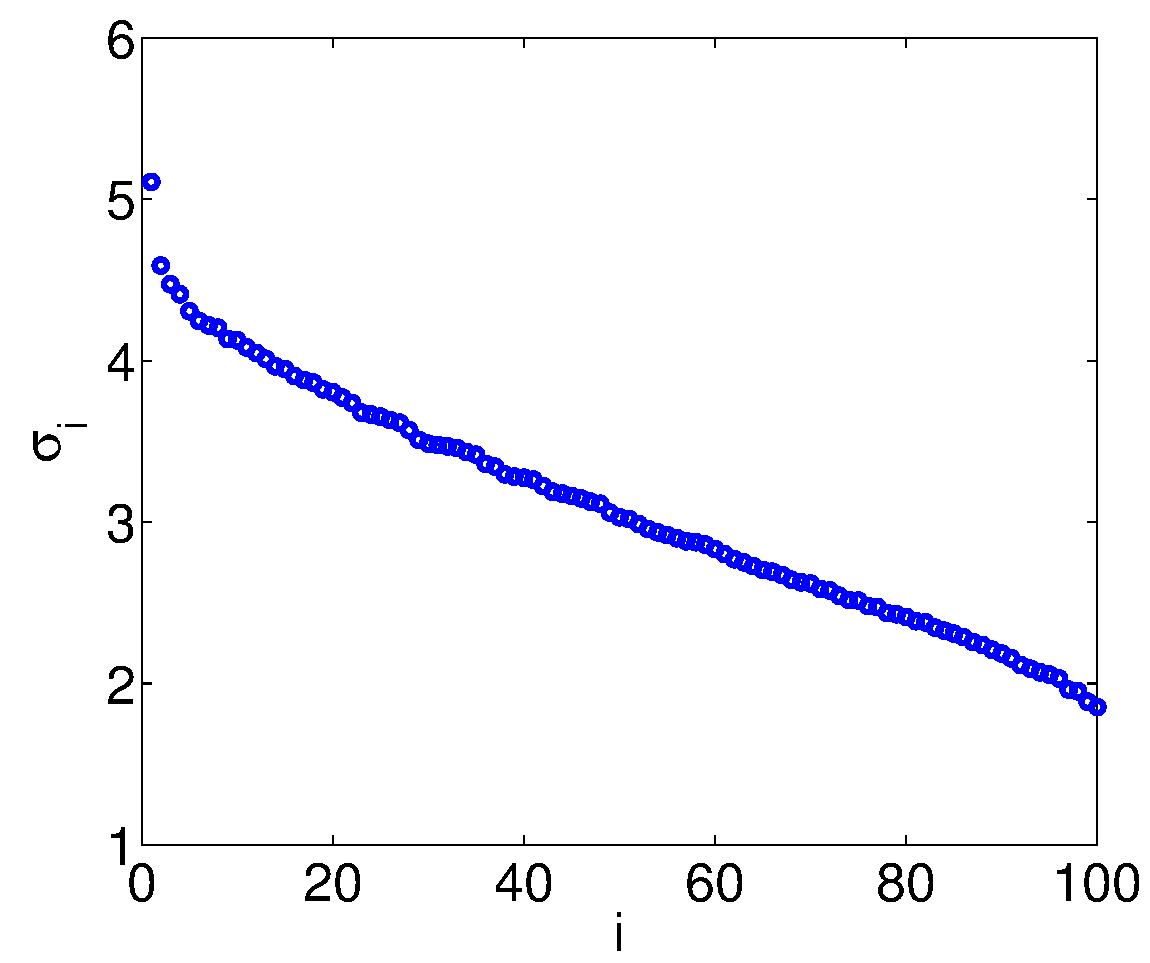
\includegraphics[width=0.3\textwidth]{chpt7_svd_proj/figs/motiv_gauss_1.pdf}
  }
  \subfigure[$\widetilde{X}$]{
    \label{fig:chpt7:motiv_full2}
    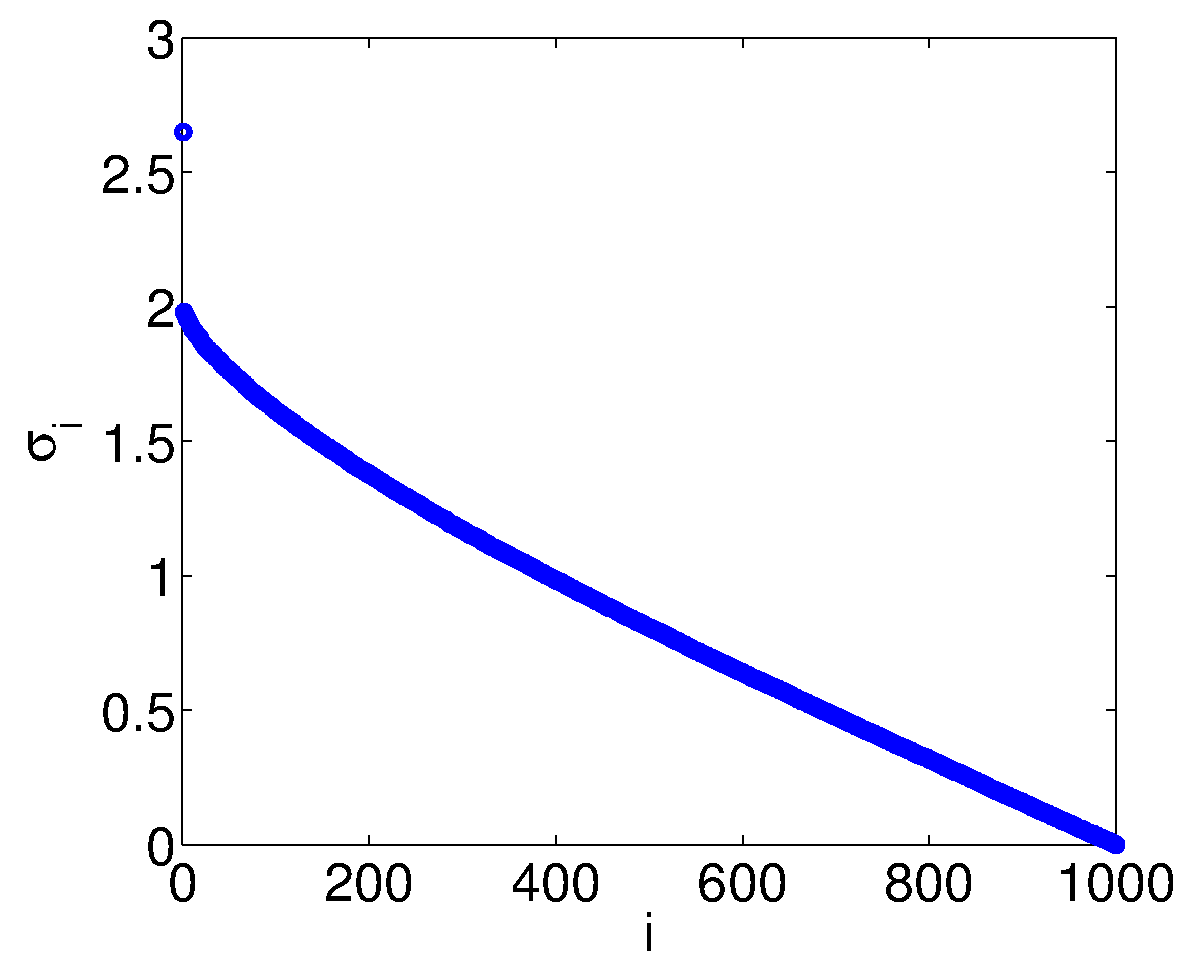
\includegraphics[width=0.3\textwidth]{chpt7_svd_proj/figs/motiv_full_2.pdf}
  }
  \subfigure[$Q^H\widetilde{X}$]{
    \label{fig:chpt7:motiv_orth2}
    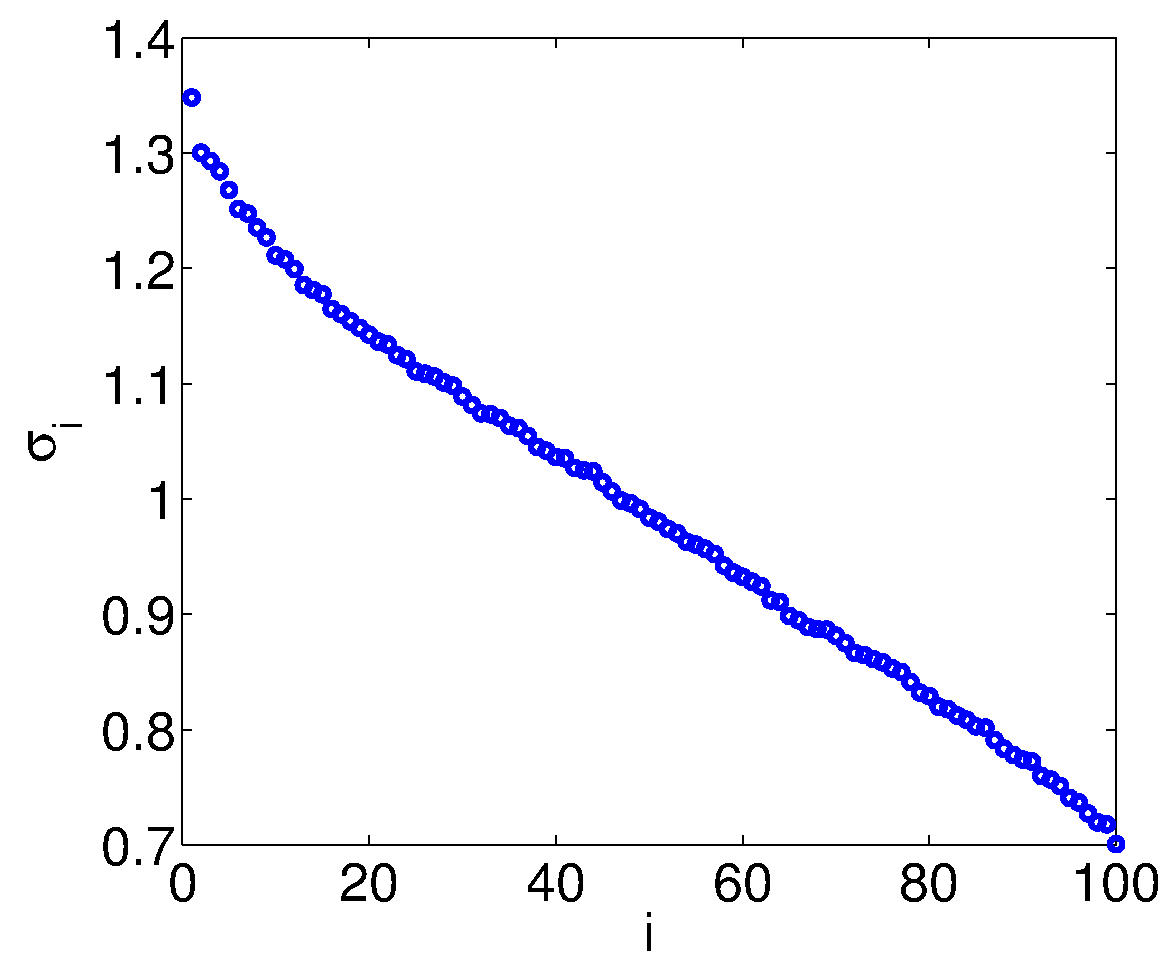
\includegraphics[width=0.3\textwidth]{chpt7_svd_proj/figs/motiv_orth_2.pdf}
  }
  \subfigure[$G^H\widetilde{X}$]{
    \label{fig:chpt7:motiv_gauss2}
   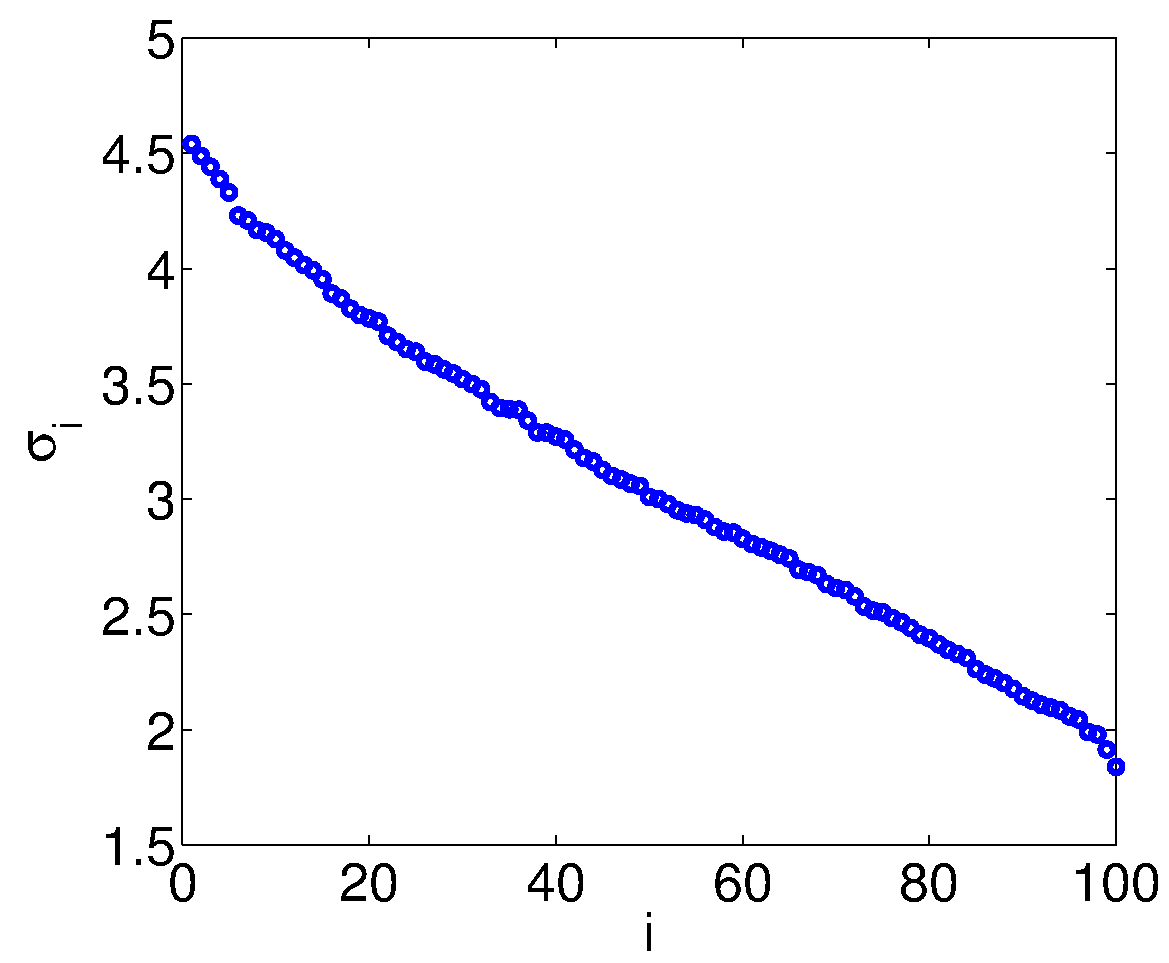
\includegraphics[width=0.3\textwidth]{chpt7_svd_proj/figs/motiv_gauss_2.pdf}
  }
  \caption{ Rank-1 simulation setting where $n=1000$, $m=100$, $N=1000$, and
    $r=1$. (a)-(c) set $\theta=\theta_x=\theta_y=4$. (d)-(f) set
    $\theta=\theta_x=\theta_y=2.2$. Each subfigure plots the singular value spectra for a
    particular matrix. (a) and (d) plot the spectra of $\widetilde{X}$. (b) and (e) plot
    the spectra of the matrix after applying an orthogonal projection matrix. (c) and (f)
    plot the spectra of the matrix after applying a Gaussian projection matrix. We observe
    that for a large SNR ((a) - (c)), the largest singular value of all matrices separate,
    indicating the presence of the rank-1 signal. However, for smaller SNR ((d) - (f)),
    the largest singular value using the unitary projection matrix separates while that
    using the Gaussian projection matrix does not.}
  \label{fig:chpt7:motivation}
\end{center}
\end{figure*}
\end{comment}

\section{Main Results}\label{sec:chpt7:main_results}

Our main result characterizes the asymptotic behavior of the largest
singular values of the projection matrices defined in (\ref{eq:chpt7:yn}). We begin with
the following assumptions and definitions. 

\begin{Assum}\label{assum:x_limit}
The probability measures $\mu_{X_n}$, $\mu_{G_n}$, and $\mu_{Q_n}$ converge almost surely
weakly to non-random compactly supported probability measures $\mu_X$,$\mu_G$, and
$\mu_Q$, respectively.  
\end{Assum}

\begin{Def}
Let $M_n^G = G_n^HX_n$ be the product of the random matrices $G_n$ and $X_n$ and let
$M_n^Q=Q_n^HX_n$ be the product of the random matrices $Q_n$ and $X_n$.
\end{Def}

\begin{Assum}\label{assum:m_limit}
The probability measure $\mu_{M_n^G}$ converges almost surely weakly to a non-random
compactly supported probability measure $\mu_{M_G}$. The probability measure $\mu_{M_n^Q}$
converges almost surely weakly to a non-random compactly supported probability measure
$\mu_{M_Q}$.  
\end{Assum}

\begin{Assum}
Let $a_G$ be the infimum of the support $\mu_{M_G}$. The smallest singular value of $M_n^G$
converges almost surely to $a_G$. Let $a_Q$ be the infimum of the support $\mu_{M_Q}$. The
smallest singular value of $M_n^Q$ converges almost surely to $a_Q$.
\end{Assum}

\begin{Assum}\label{assum:m_b}
Let $b_G$ be the supremum of the support $\mu_{M_G}$. The largest singular value of $M_n^G$
converges almost surely to $b_G$. Let $b_Q$ be the supremum of the support $\mu_{M_Q}$. The
largest singular value of $M_n^Q$ converges almost surely to $b_Q$.
\end{Assum}

With these assumptions and definitions, we now state our main results
about the almost sure limit of the largest singular values of the projection matrices
defined in (\ref{eq:chpt7:yn}). 

\begin{Th}\label{thm:svd_proj}
Let $Y_n$ be the projection of $\widetilde{X}_n$ onto either $G_n$ or $Q_n$ as in
(\ref{eq:chpt7:yn}). The largest $r$ singular values of the $m\times N$ matrix $Y_n$ exhibit the
following behavior as $n,m,N\to\infty$ with $n/N\to c_1$ and $m/n\to c_2$. We have that
for each fixed $1\leq i\leq r$, $\sigma_i\left(Y_n\right)$ solves
\beq\label{eq:chpt7:solution}
\sigma_i^2\varphi_F(\sigma_i)\varphi_H(\sigma_i) = \frac{1}{\theta_i^2},
\eeq
where
\be\ba
&\varphi_{F}(\sigma_i)\convas-\E{xm_{\mu_{RS|R}}\left(\sigma_i^2,x\right)}_{\mu_R}\\
&\varphi_{H}(\sigma_i)\convas-\frac{n}{N}m_{M_3}(\sigma_i^2) - \frac{1}{\sigma_i^2}\frac{n-N}{N}
\ea\ee
where $m_{\mu_M}$ is the Stieltjes transform of a matrix $M$ defined as
\be
m_{\mu_{M}}(z)\int\frac{1}{x-z}\mu_{M}(x),
\ee
and $\mu_R$ is the limiting eigenvalue density of either $G_nG_n^H$ or $Q_nQ_n^H$,
$\mu_S$ is the limiting eigenvalue density of $X_nX_n^H$, $m_{\mu_{RS|S}}$ is the
Stieltjes transform of the limiting conditional density
and $m_{\mu_{M_3}}$ is the
Stieltjes transform of $G_nG_n^HX_nX_n^H$ or $Q_nQ_n^HX_nX_n^H$. When using $G_n$,
$m_{\mu_{RS|S}}(z,x)$ solves the following equation
\beq\label{eq:chpt7:ugly}\begin{split}
  0 = &\left(-n^2z^2\right)\left(m_{\mu_{RS|S}}(z,x)\right)^3 + Nm \\& +\left(Nnz+mnz-2n^2z\right)
  \left(m_{\mu_{RS|S}}(z,x)\right)^2 \\&+\left(Nn+mn+Nmz-n^2-Nm\right) m_{\mu_{RS|S}}(z,x).
\end{split}
\eeq
\end{Th}

When using the Gaussian projection matrix, $G_n$, we do not get a closed form of the top
singular values. Solving (\ref{eq:chpt7:ugly}) for $m_{\mu_{RS|S}}(z,x)$ is unwieldy as we
must solve a cubic polynomial. Furthermore, we must take the expectation of the resulting
solution with respect to the distribution $\mu_R$. To solve the expressions $\varphi_F$
and $\varphi_H$ when using a Gaussian projection matrix, we use RMTool
\cite{rao2008polynomial}. We note that this process still yields an analytic
solution, although not closed form. However, when using a unitary projection matrix, we do
get a closed form expression for the largest singular values.

\begin{Corr}\label{corr:svd_proj_unitary}
When $Y_n$ is a generated using a unitary matrix $Q_n$, we have that
for each fixed $1\leq i\leq r$,
\be
\sigma_i \convas \begin{cases} \sqrt{\frac{c_1}{\theta_i^2}+c_2\theta_i^2+1+c_1c_2} & \text{if }
  \theta_i\geq\left(\frac{c_1}{c_2}\right)^{1/4}\\ \sqrt{c_1c_2} +1 & \text{if }
    \theta_i<\left(\frac{c_1}{c_2}\right)^{1/4} \end{cases}.
\ee
\end{Corr}

This corollary nicely gives the almost sure limit of the top singular values as a function
of the system parameters $n$, $m$, $N$, and $\theta_i$. This corollary also makes contact
with a natural phase transition. When the SNR of a component is below a critical value
depending only on $n,m,N$, the corresponding top singular value behaves as if $Y_n$ is a
noise only matrix. Such phase transitions appear in other matrix analyses (see
\cite{paul2007asymptotics,
  benaych2011eigenvalues,asendorf2013performance,benaych2012singular}). Similarly, we may
solve for the phase transition when using a Gaussian matrix, although we do not get a
closed form expression as we do in the unitary case.  We state a more general version of
this phase transition in the form of the following corollary.

\begin{Corr}\label{corr:svd_proj_pt}
When 
\be
\theta_i \leq \theta_{\text{crit}} = \frac{1}{b\sqrt{\varphi_F(b)\varphi_H(b)}}
\ee
then 
\be
\sigma_i\convas b,
\ee
where $b$ is either $b_Q$ or $b_G$ depending on our projection matrix. 
\end{Corr}

When a component's SNR is below a critical SNR (given in the corollary), then the
corresponding singular value of $Y_n$ does not separate from its noise distribution. In
this scenario, this signal is not detectable. 

\section{Empirical Results}\label{sec:chpt7:emp_res}

In this section we verify the singular value prediction given in (\ref{eq:chpt7:solution})
that relies on the asymptotic approximations $\varphi_F$ and $\varphi_H$. We consider two
different types of projection matrices. In the first setting, we use a matrix $G_n$ with
independent $\mathcal{N}(0,1)$ entries. In the second setting, we use a unitary matrix $Q_n$
such that $Q_n^HQ_n=I_m$. In both settings, we let the noise matrix $X_n$ be an appropriately
scaled random Gaussian matrix whose entries are independent standard Gaussian random
variables. 

\subsection{Gaussian Projection, $G$}

In this setting, $R=GG^H$ and $S=XX^H$ are independent Wishart random matrices with
parameters $c_2 = \frac{n}{m}$ and $c_1=\frac{n}{N}$. To compute $\varphi_F$ and $\varphi_H$,
we use RMTool \cite{rao2008polynomial}. We numerically approximate the expected value
using RMTool to approximate the density of $R$ and to compute the Stieltjes transform of
the kernel. We use 2500 points in the approximation. To compute $\varphi_H$, We consider
the matrix $M_2=GG^HXX^H=RS$, which is a product of Wishart matrices. This is desirable as
we can use RMTool to compute the Stieltjes transform as above for $\varphi_H$.  

Figure \ref{fig:chpt7:gauss_pred} shows the performance of our theoretical prediction when
using a Gaussian projection matrix, $G$, for a rank-1 setting with a fixed $n=1000$,
$N=1220$, $m=100$. In our empirical setup, we generate 500 matrices from
(\ref{eq:chpt7:data_model}) and 500 noise only matrices. We then generate a random $G$
selected as above. The figure plots the empirical and theoretically predicted top singular
value for a number of $\theta_1=\theta$. As evident in the figure, the theoretical
prediction does a good job except. 

In Figure \ref{fig:chpt7:gauss_like_pred} we consider a Gaussian-like projection matrix
for the same rank-1 setting as Figure \ref{fig:chpt7:gauss_pred}. For this figure, the
entries of $G$ are 
\beq\label{eq:chpt7:g_like}
G_{ij} = \begin{cases} 1 & \text{w.p. } 1/2\\ -1 & \text{w.p. } 1/2\end{cases}
\eeq
so that they have zero mean and unit variance. We see that the theoretical prediction from
(\ref{eq:chpt7:solution}) for the Gaussian setting is still valid for this Gaussian-like
projection matrix.

\begin{figure}
  \begin{center}
    \subfigure[Gaussian $G$]{
      \label{fig:chpt7:gauss_pred}
      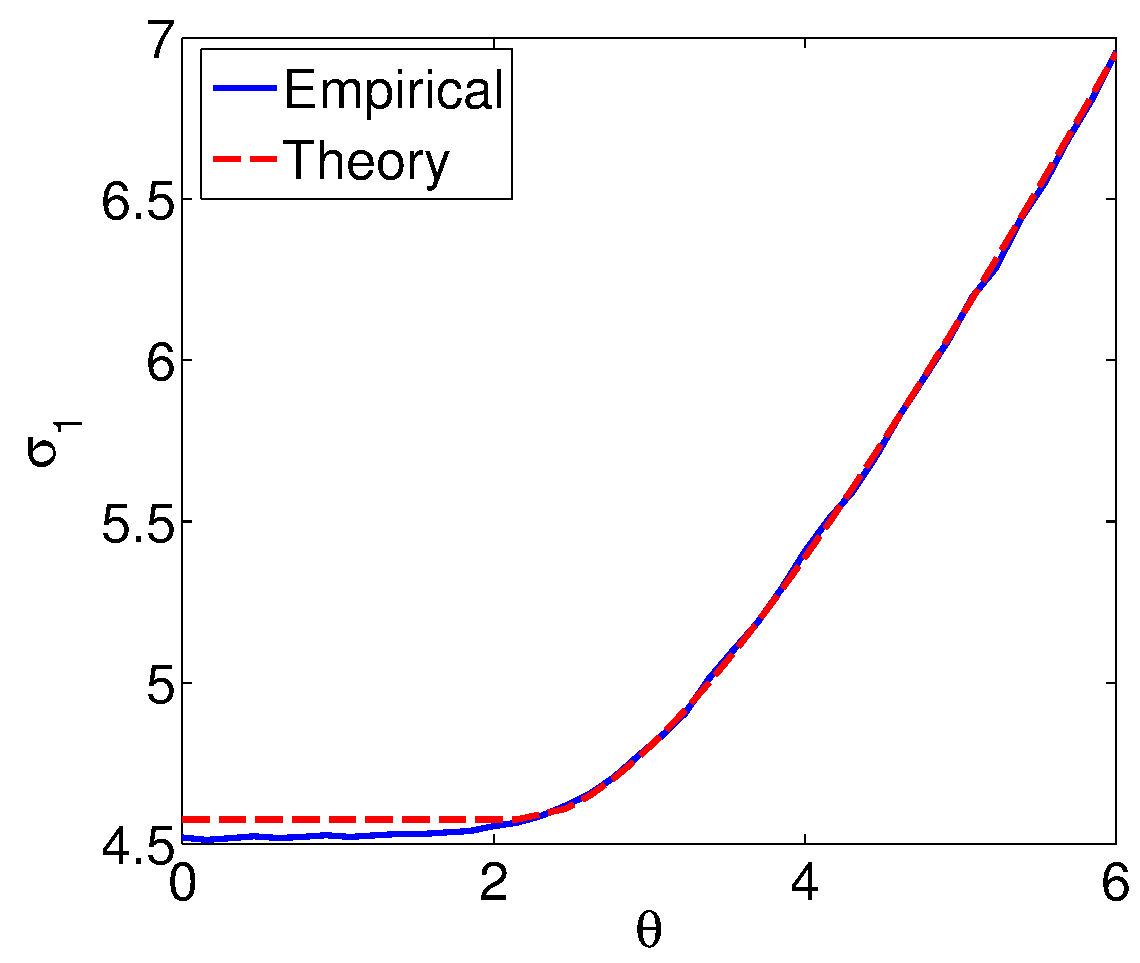
\includegraphics[width=0.35\textwidth]{chpt7_svd_proj/figs/gauss_sv_pred.pdf}
    }
    \subfigure[Gaussian-like $G$]{
      \label{fig:chpt7:gauss_like_pred}
      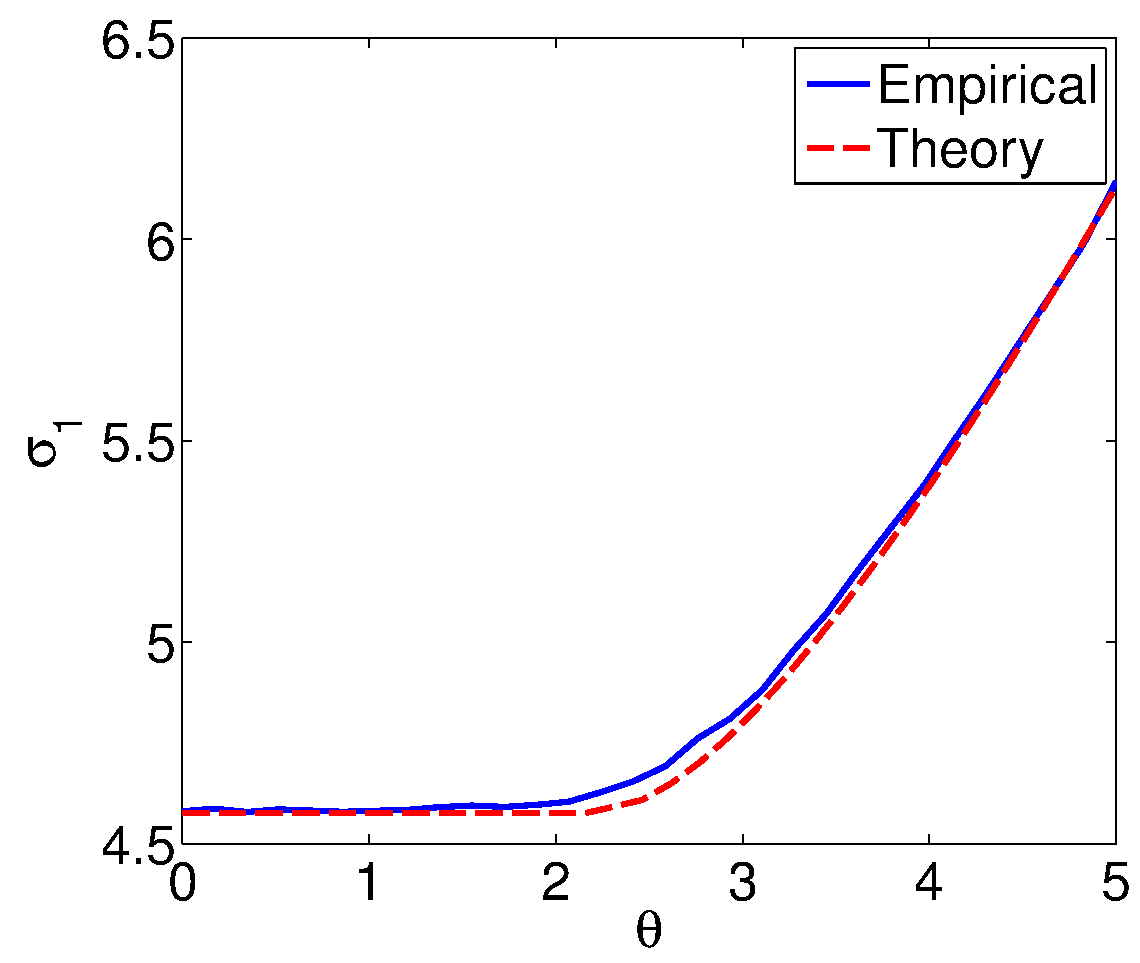
\includegraphics[width=0.35\textwidth]{chpt7_svd_proj/figs/gauss_sweep.pdf}
    }
    \caption{Singular value prediction for Gaussian $G$ and $X$ for a rank-1 setting
      with fixed $n=1000$, $N=1220$ and $m=100$. The theoretical prediction uses
      (\ref{eq:chpt7:solution}) with approximations using RMTool. Empirical results are
      averaged over 500 trials. (a) Gaussian $G$ (b) Entries of $G$ are from
      (\ref{eq:chpt7:g_like}).}
    \label{fig:chpt7:gauss_sv}
  \end{center}
\end{figure}

We then explore the accuracy of the phase transition boundary for the Gaussian setting in
Figure \ref{fig:chpt7:gauss} by plotting the KS-statistic between the largest singular
values from these 500 signal and noise only matrices for $n=1000$. Figure
\ref{fig:chpt7:gauss1} sweeps over $\theta$ and $N$ while Figure \ref{fig:chpt7:gauss2} sweeps
over $\theta$ and $m$. In both figures, we plot our theoretical phase transition prediction
in solid white line. Using a dashed white line, we plot the theoretical phase transition
when no projection is used; this is $\theta=\left(\frac{n}{N}\right)^{1/4}$.

From this figure, we observe that the phase transition prediction is very
accurate. Similarly we notice that the phase transition when using the Gaussian projection
is significantly worse that that when not projecting. Figure \ref{fig:chpt7:gauss1} sets
$m=100$ so that we reduce our SVD dimension by one order of magnitude. Interestingly, and
perhaps most importantly, when using a Gaussian projection matrix, setting $m=n=1000$
results in worse performance than the non-projecting case even though we aren't reducing
the dimension of the problem. This is evident in Figure \ref{fig:chpt7:gauss1}.


\begin{figure}
\begin{center}
  \subfigure[KS Statistic - $N$,$\theta$ sweep]{
    \label{fig:chpt7:gauss1}
    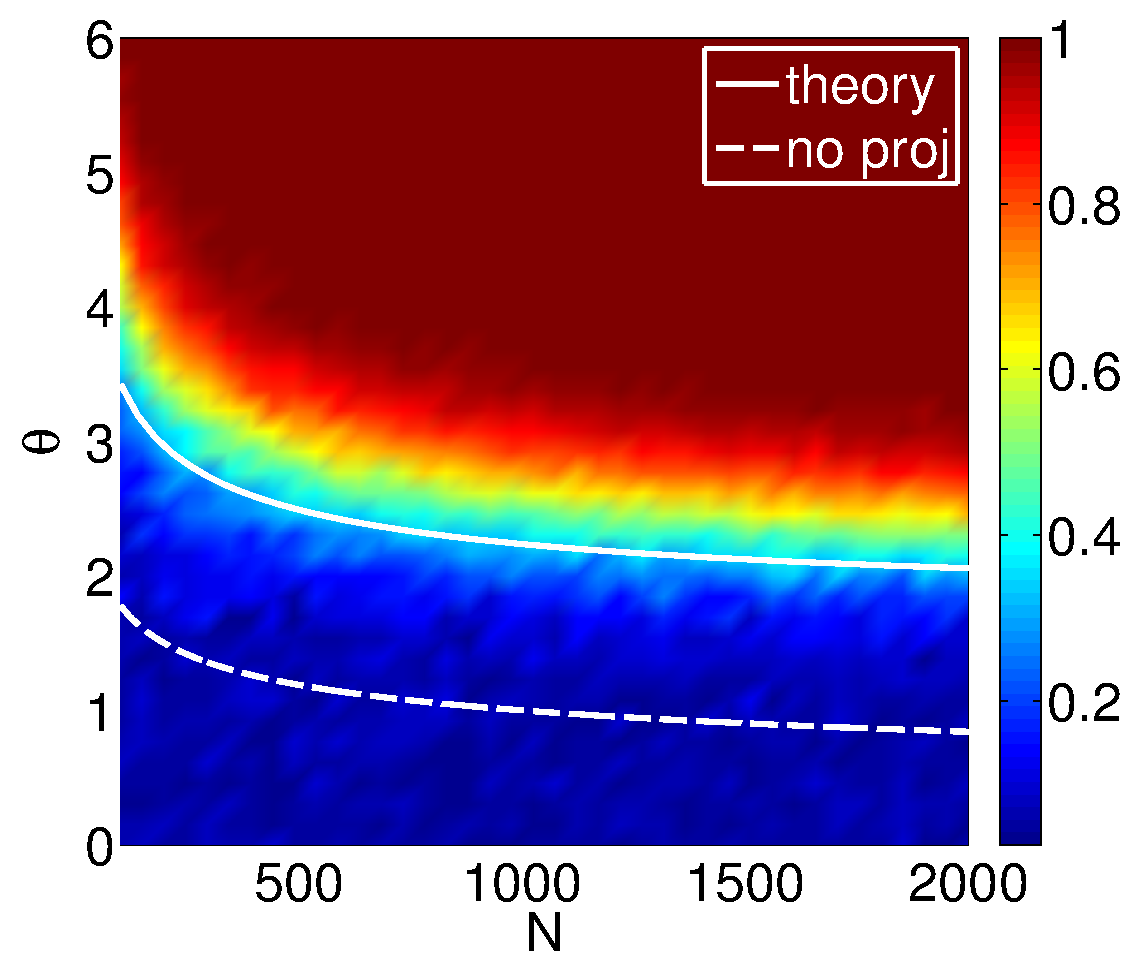
\includegraphics[width=0.4\textwidth]{chpt7_svd_proj/figs/ks11.pdf}
  }
  \subfigure[KS Statistic - $m$,$\theta$ sweep]{
    \label{fig:chpt7:gauss2}
    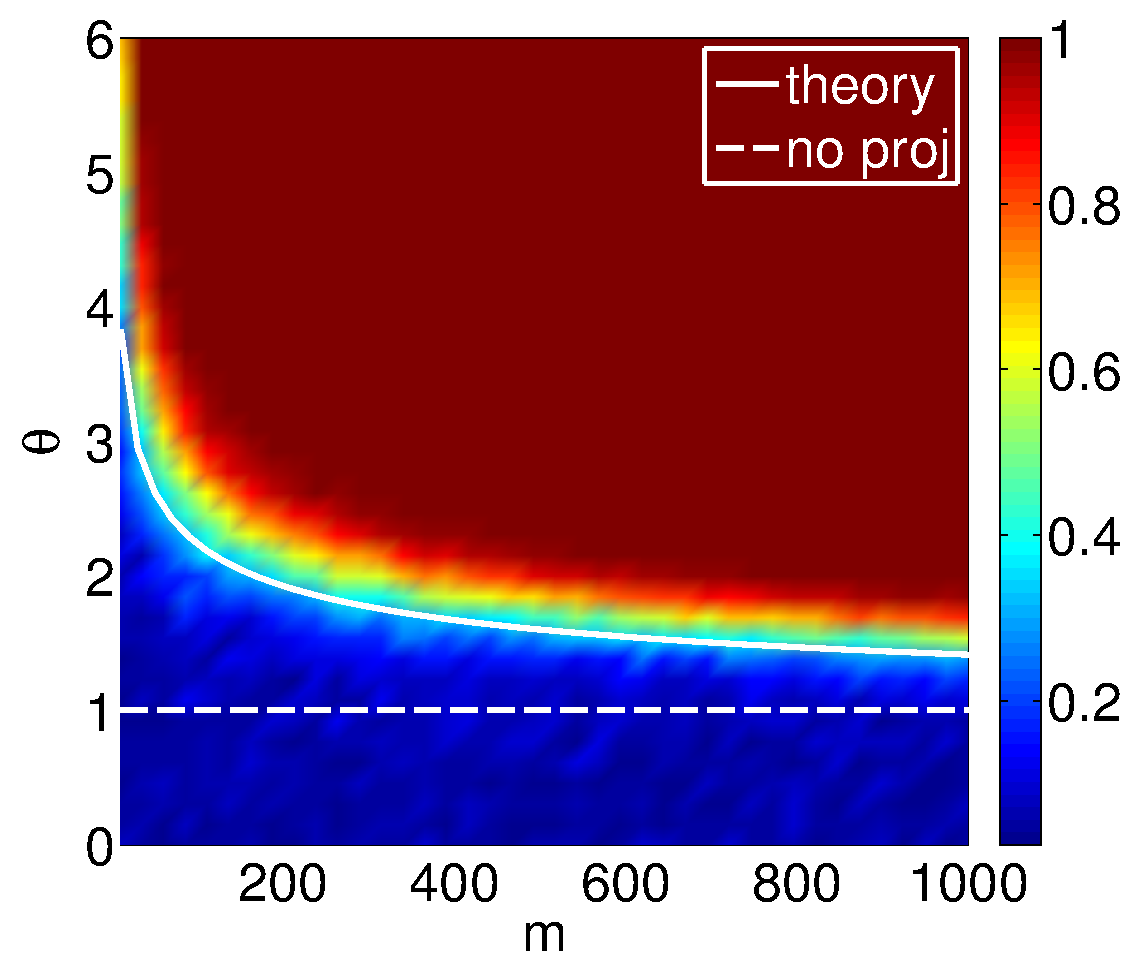
\includegraphics[width=0.4\textwidth]{chpt7_svd_proj/figs/ks21.pdf}
  }
%  \subfigure[Maximum singular value - $N$,$\theta$ sweep]{
%    \label{fig:chpt7:gauss3}
%   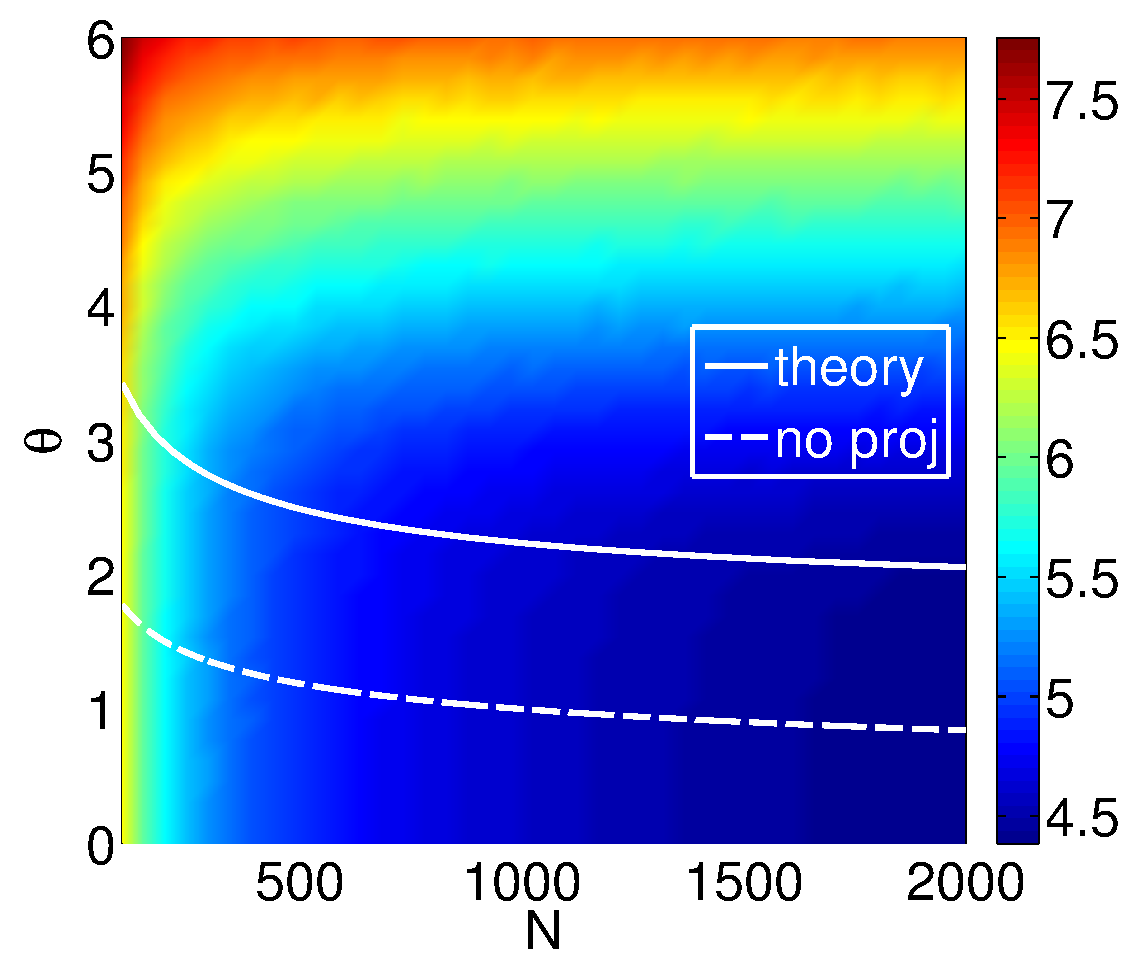
\includegraphics[width=0.357\textwidth]{chpt7_svd_proj/figs/maxsv11.pdf}
%  }
%  \subfigure[Maximum singular value - $m$, $\theta$ sweep]{
%    \label{fig:chpt7:gauss4}
%    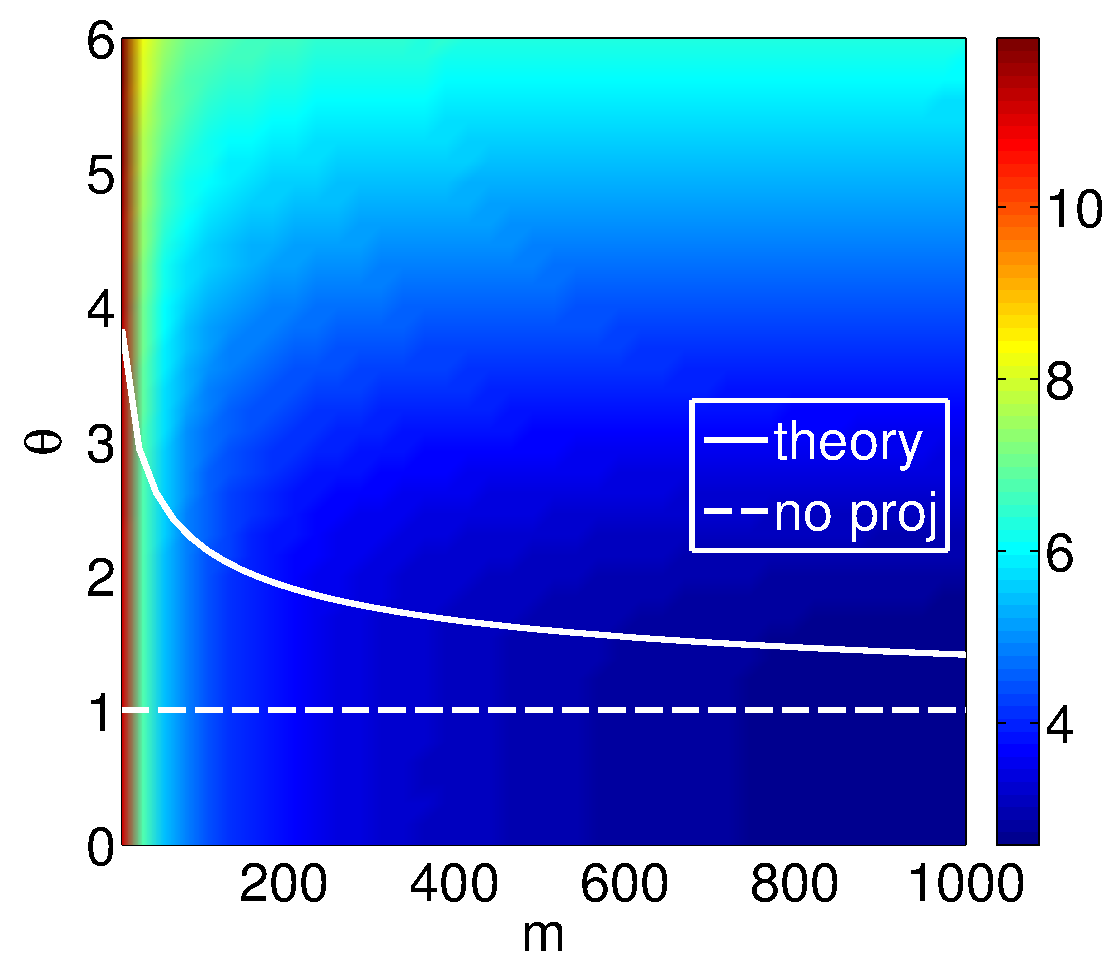
\includegraphics[width=0.357\textwidth]{chpt7_svd_proj/figs/maxsv21.pdf}
%  }
%  \subfigure[Singular Vector accuracy $N$,$\theta$ sweep]{
%    \label{fig:chpt7:gauss5}
%   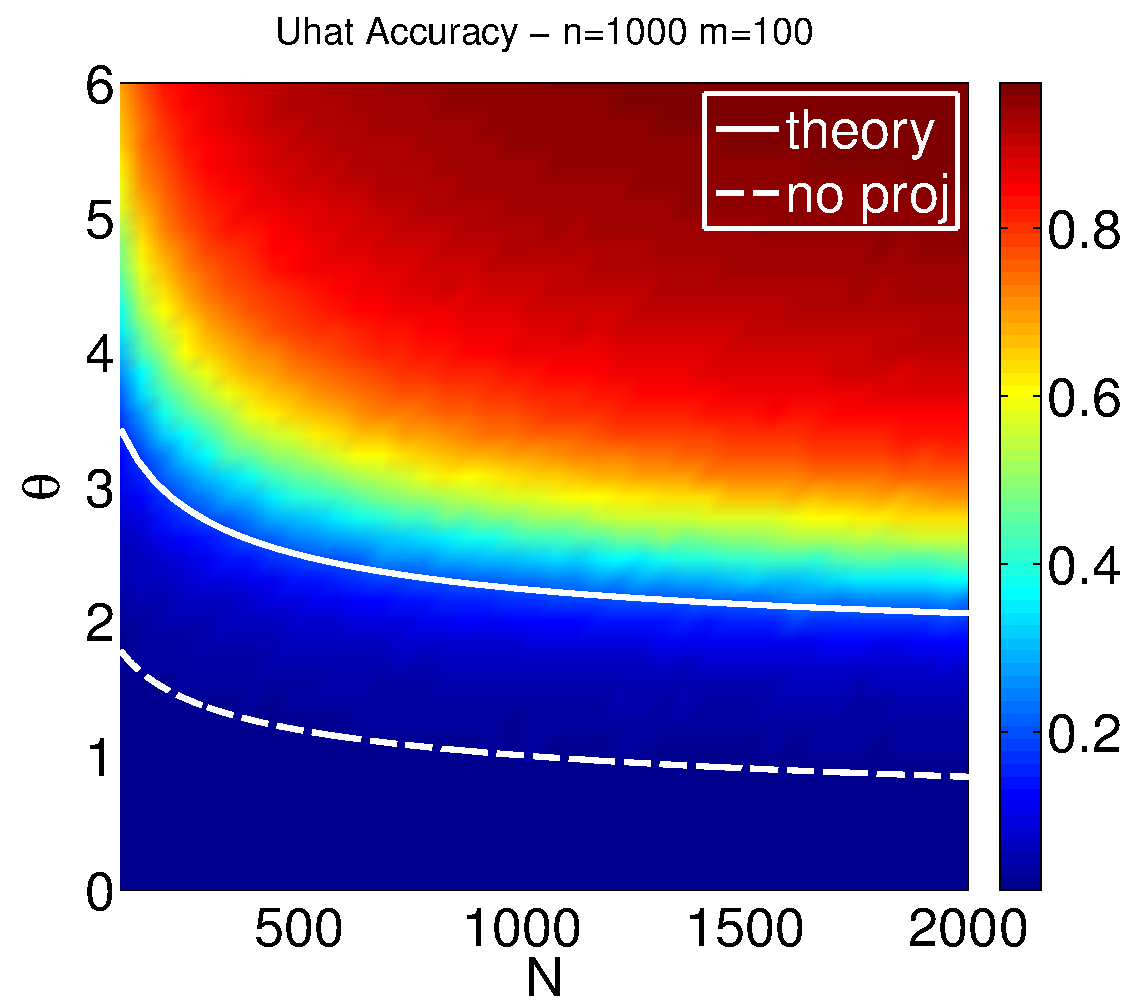
\includegraphics[width=0.357\textwidth]{chpt7_svd_proj/figs/uhat11.pdf}
%  }
%  \subfigure[Singular Vector accuracy $m$,$\theta$ sweep]{
%    \label{fig:chpt7:gauss6}
%    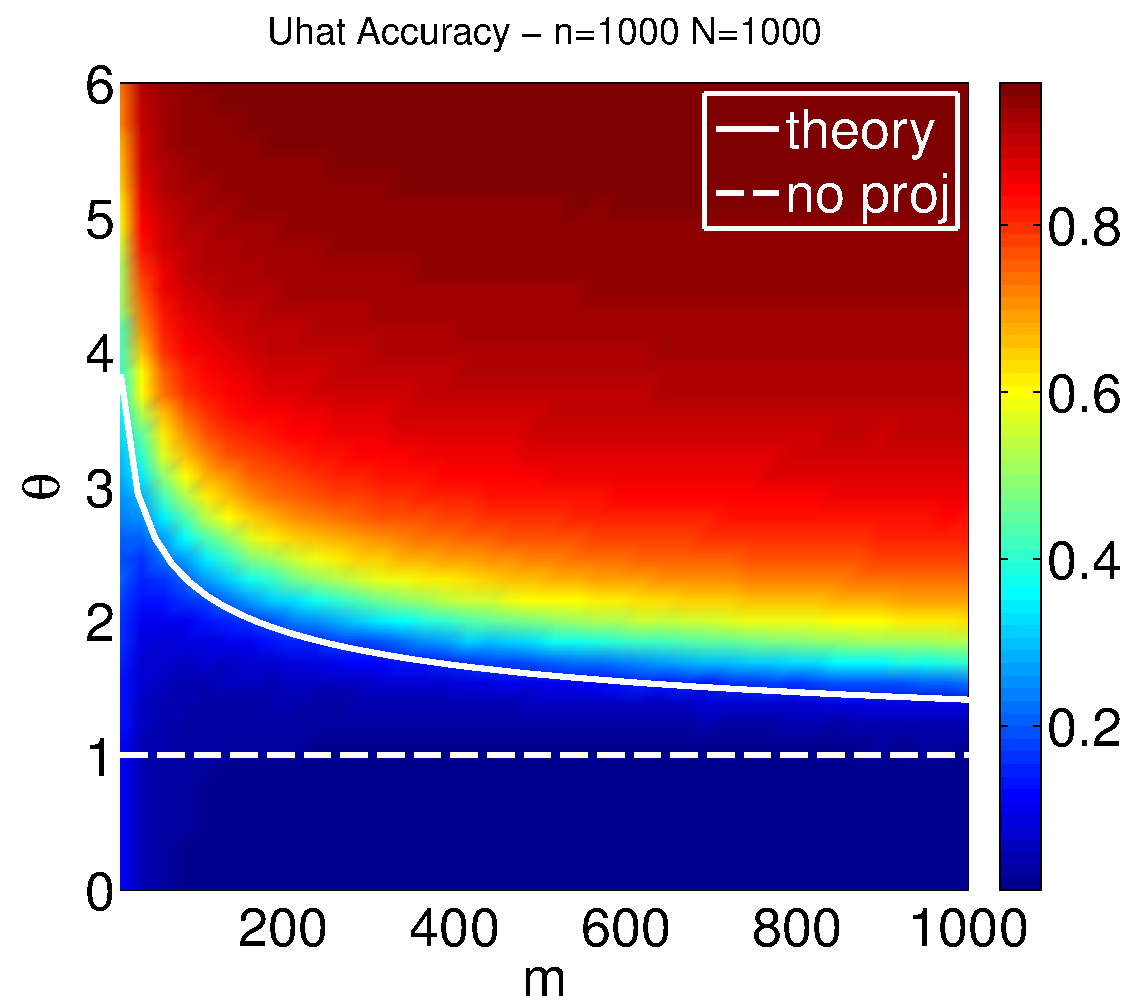
\includegraphics[width=0.357\textwidth]{chpt7_svd_proj/figs/uhat21.pdf}
%  }
  \caption{Accuracy of theoretical phase transition prediction for Gaussian $G$ and $X$
    for a rank-1 setting with fixed $n=1000$. The theoretical prediction uses
    (\ref{eq:chpt7:solution}) with approximations using RMTool. Figures plot the KS
    statistic between singular values generated from 500 signal bearing and 500 noise only
    matrices. (a) Sweeps over both $\theta$ and $N$ for a fixed $m=100$. (b) Sweeps over
    $\theta$ and $m$ for a fixed $N=1000$.}
  \label{fig:chpt7:gauss}
\end{center}
\end{figure}

\subsection{Unitary Projection, $Q$}

In this setting, we use a unitary projection matrix $Q$ using a QR decomposition of a
random matrix. Figure \ref{fig:chpt7:ortho_pred} plots the performance of our theoretical
prediction for a rank-1 setting with a fixed $n=1000$, $N=1220$, $m=100$. In our empirical
setup, we generate 500 matrices from (\ref{eq:chpt7:data_model}) and 500 noise only
matrices. We then generate a random $Q$ selected as above. The figure plots the empirical
and theoretically predicted top singular value for a number of $\theta_1=\theta$. The
theoretical prediction uses the result from Corollary \ref{corr:svd_proj_unitary} and does
an excellent job at the singular value prediction.

In Figure \ref{fig:chpt7:fourier_pred}, we consider a specific choice of unitary
matrix. Here, we randomly select columns from the $n\times n$ discrete Fourier matrix $F$
with entries  
\beq\label{eq:chpt7:fourier}
F_{kj} = \frac{1}{\sqrt{n}}\exp\left\{\frac{-2\pi i (k-1)(j-1)}{n}\right\}
\eeq
for $k=1\dots,n$ and $j=1,\dots,n$. To generate $Q$ we then select $m$ columns from
$F$. We see that the theoretical prediction from Corollary \ref{corr:svd_proj_unitary}
still does an excellent job at the singular value prediction for this specific choice of
unitary matrix. 

\begin{figure}
  \begin{center}
    \subfigure[Unitary $Q$]{
      \label{fig:chpt7:ortho_pred}
      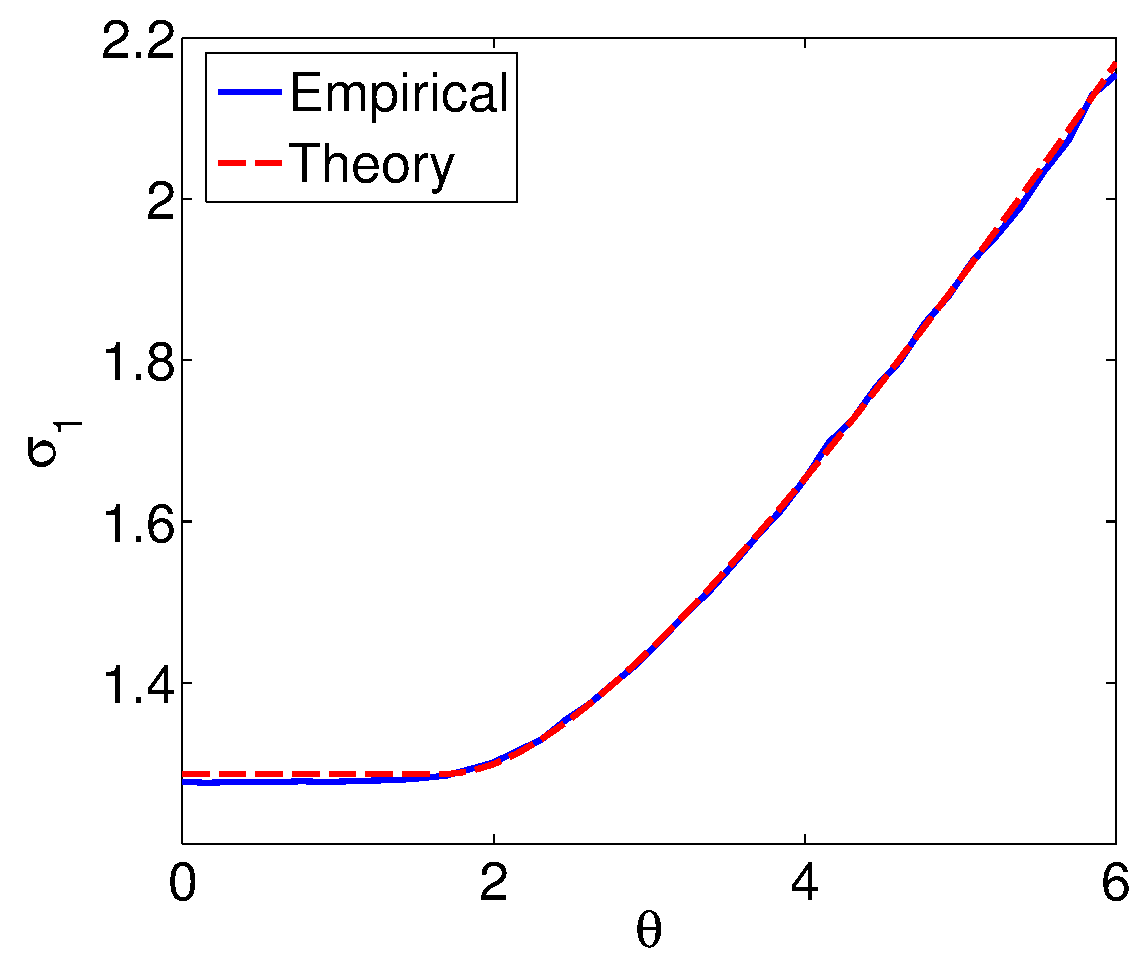
\includegraphics[width=0.35\textwidth]{chpt7_svd_proj/figs/unitary_sv_pred.pdf}
    }
    \subfigure[Fourier $Q$]{
      \label{fig:chpt7:fourier_pred}
      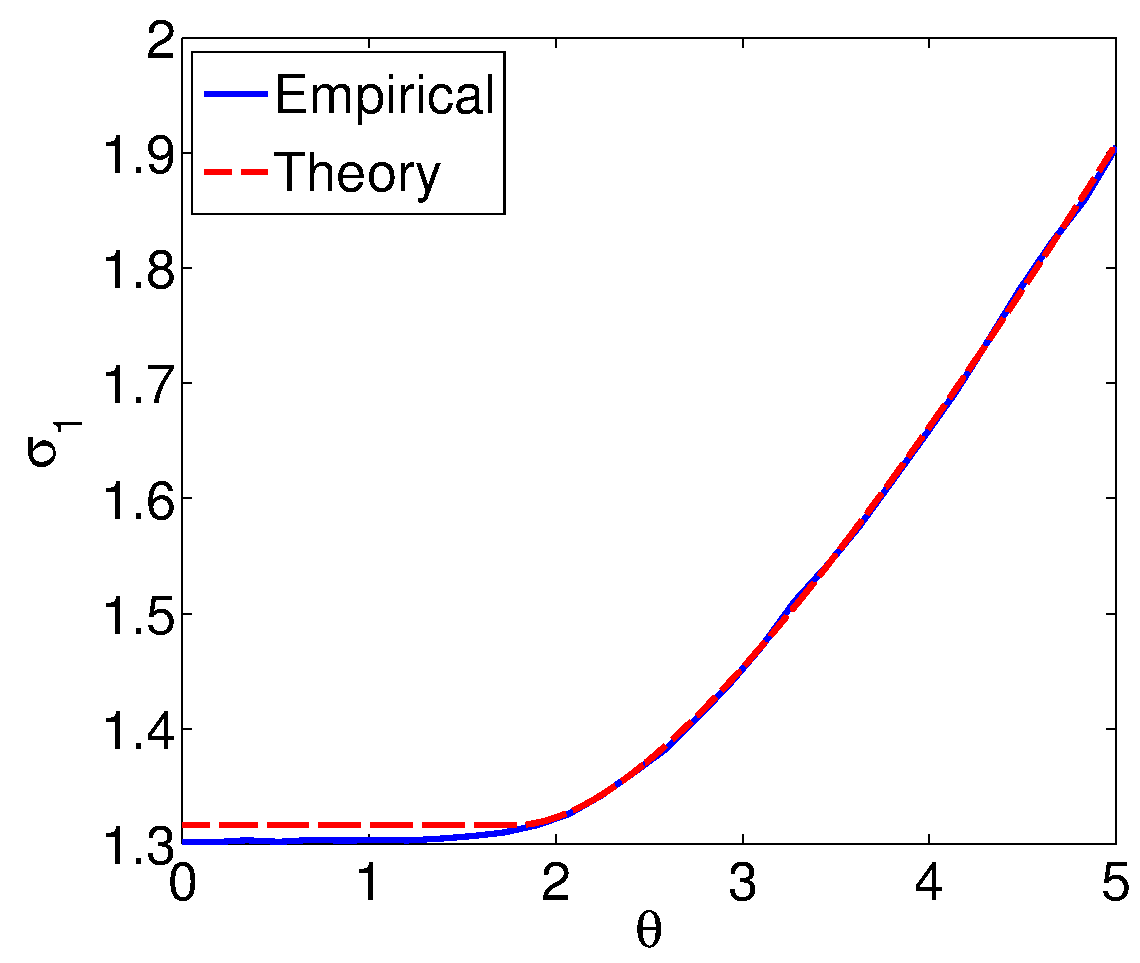
\includegraphics[width=0.35\textwidth]{chpt7_svd_proj/figs/fourier_sweep.pdf}
    }
    \caption{Singular value prediction for unitary projection matrix $Q$ and Gaussian
      noise matrix $X$ for a rank-1 setting with fixed $n=1000$, $N=1220$ and $m=100$. The
      theoretical prediction uses Corollary \ref{corr:svd_proj_unitary}. Empirical results
      are averaged over 500 trials. (a) Columns of $Q$ are from the QR decomposition of a
      random matrix. (b) Columns of $Q$ are sampled from the $n\times
      n$ discrete Fourier matrix defined in (\ref{eq:chpt7:fourier}).}
    \label{fig:chpt7:ortho_sv}
  \end{center}
\end{figure}

Figure \ref{fig:chpt7:orth_g} plots the performance of our theoretical prediction when
using a unitary projection matrix, $Q$. Our parameter sweep is the same as described for
Figure \ref{fig:chpt7:gauss}, except that here we use the phase transition prediction
given in Corollary \ref{corr:svd_proj_unitary}. Again, we notice that our phase transition
prediction is very accurate. A key observation is that for a unitary projection matrix, as
$m\to n$, the phase transition approaches that of not using a projection matrix. This is
very desirable as we don't want to suffer much performance loss for only slightly reducing
the dimension of the problem.

\begin{figure}
\begin{center}
  \subfigure[KS Statistic - $N$,$\theta$ sweep]{
    \label{fig:chpt7:ortho1}
    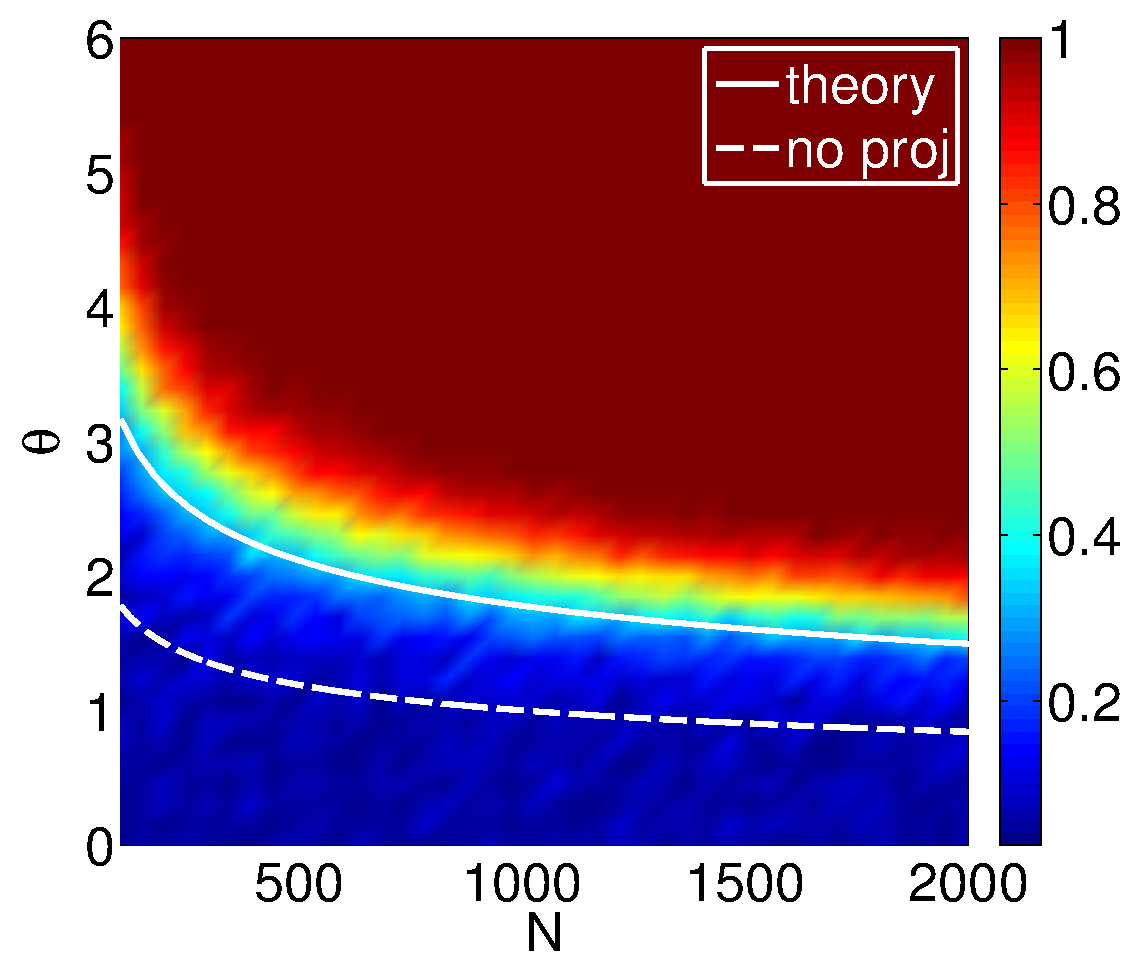
\includegraphics[width=0.4\textwidth]{chpt7_svd_proj/figs/ks12.pdf}
  }
  \subfigure[KS Statistic - $m$,$\theta$ sweep]{
    \label{fig:chpt7:ortho2}
    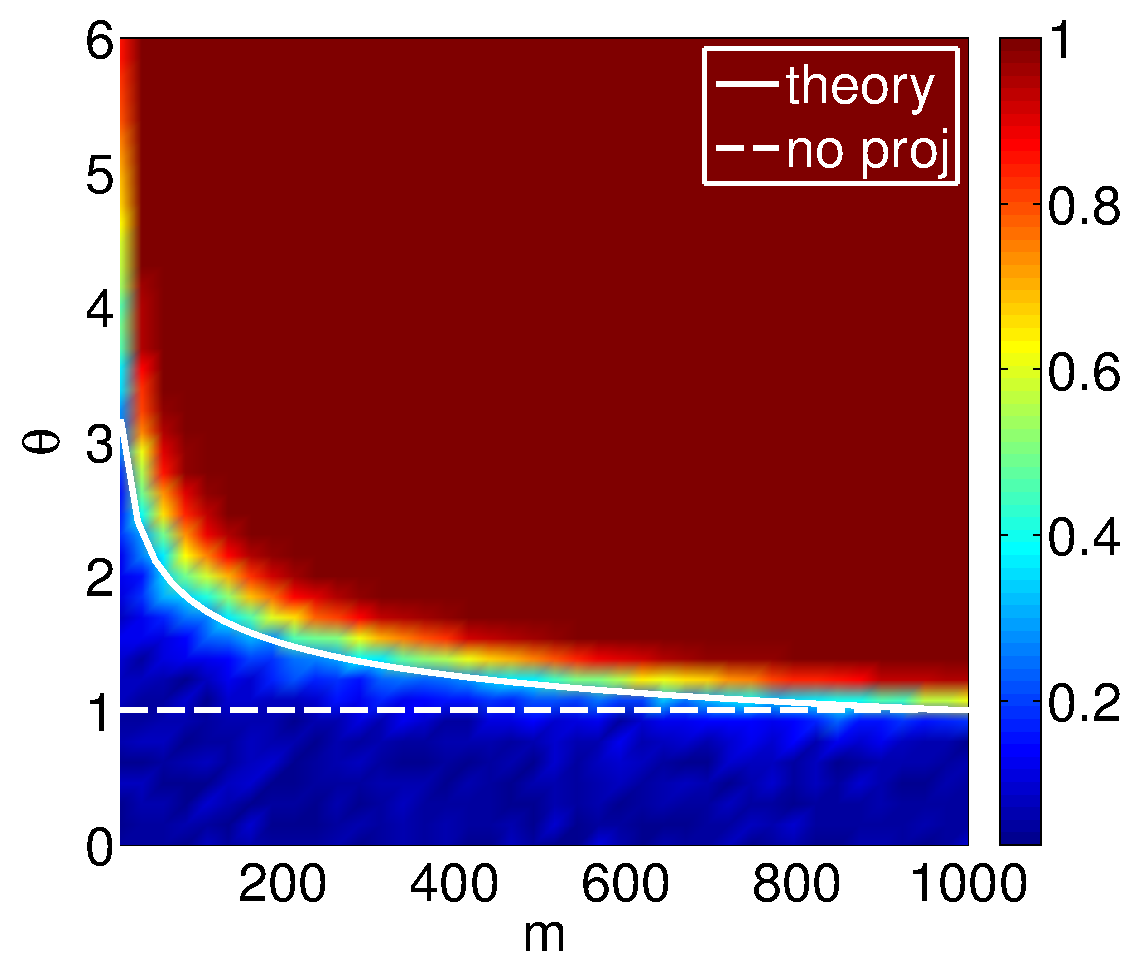
\includegraphics[width=0.4\textwidth]{chpt7_svd_proj/figs/ks22.pdf}
  }
%  \subfigure[Maximum singular value - $N$,$\theta$ sweep]{
%    \label{fig:chpt7:ortho3}
%   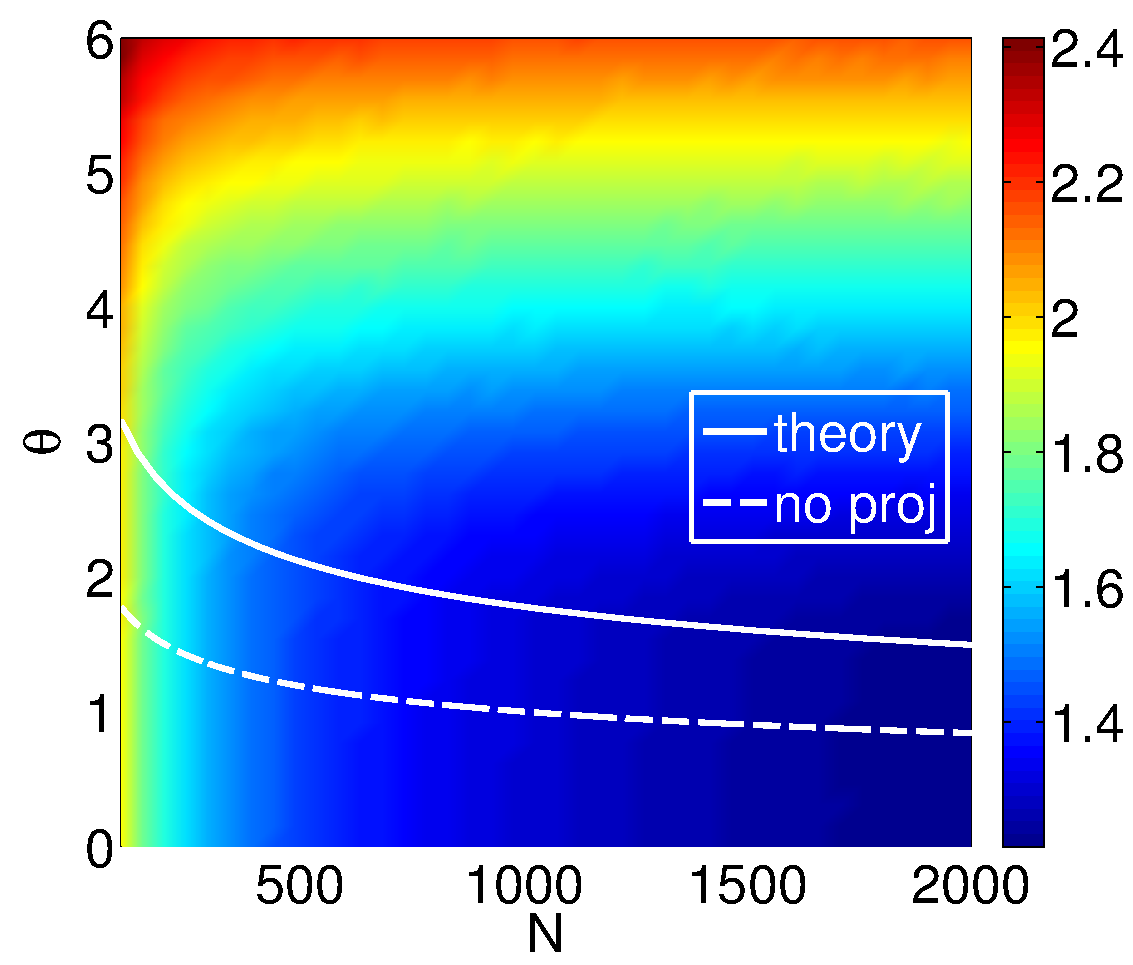
\includegraphics[width=0.357\textwidth]{chpt7_svd_proj/figs/maxsv12.pdf}
%  }
%  \subfigure[Maximum singular value - $m$, $\theta$ sweep]{
%    \label{fig:chpt7:ortho4}
%    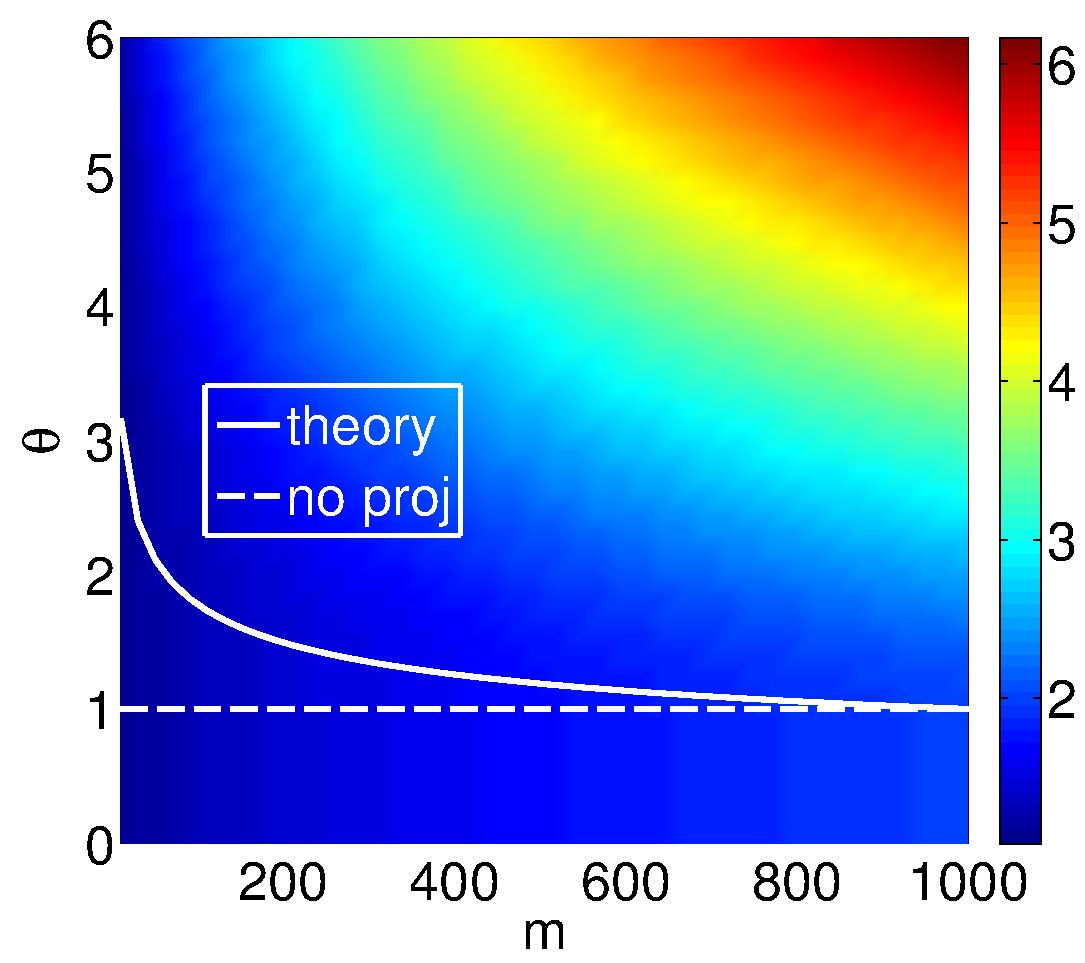
\includegraphics[width=0.357\textwidth]{chpt7_svd_proj/figs/maxsv22.pdf}
%  }
%  \subfigure[Singular Vector accuracy $N$,$\theta$ sweep]{
%    \label{fig:chpt7:ortho5}
%   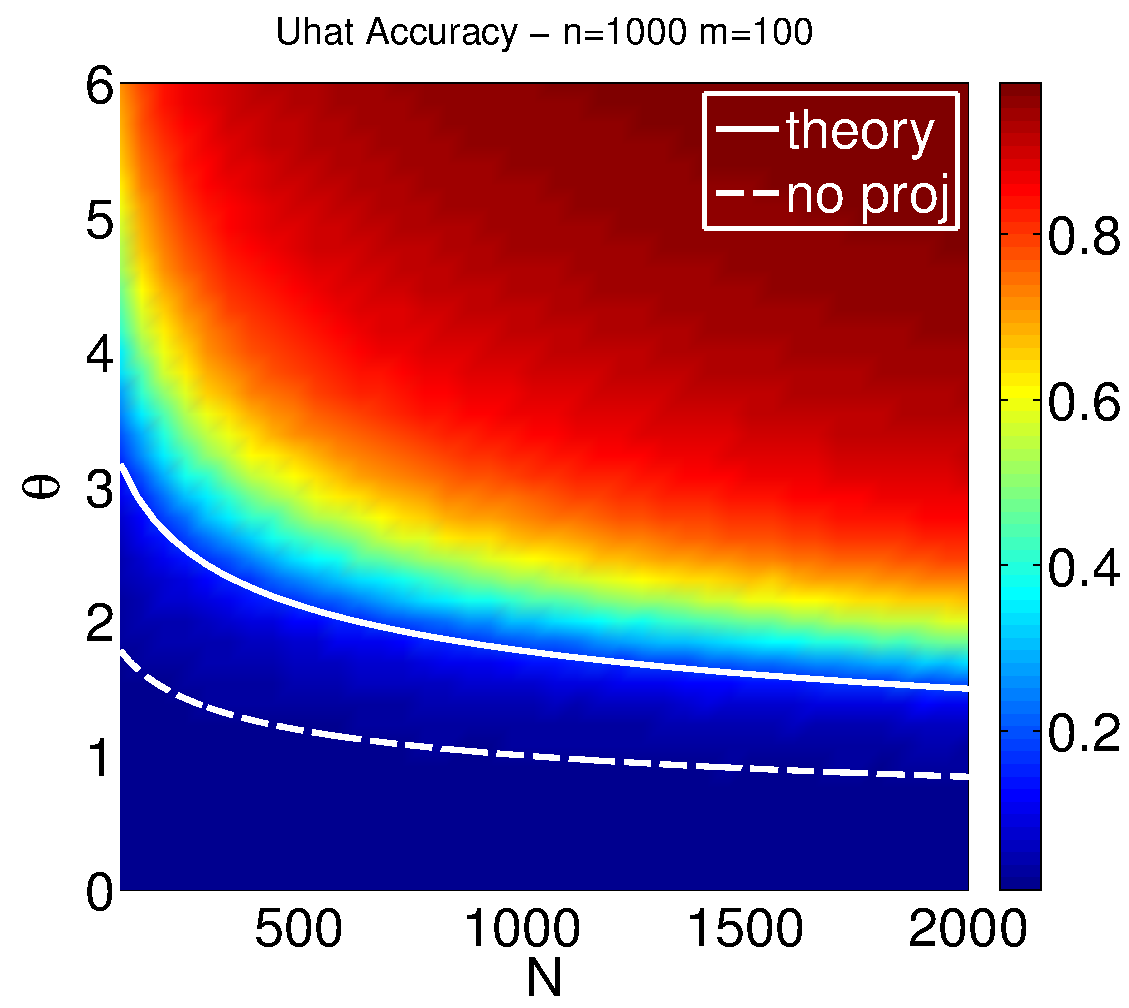
\includegraphics[width=0.357\textwidth]{chpt7_svd_proj/figs/uhat12.pdf}
%  }
%  \subfigure[Singular Vector accuracy $m$,$\theta$ sweep]{
%    \label{fig:chpt7:ortho6}
%    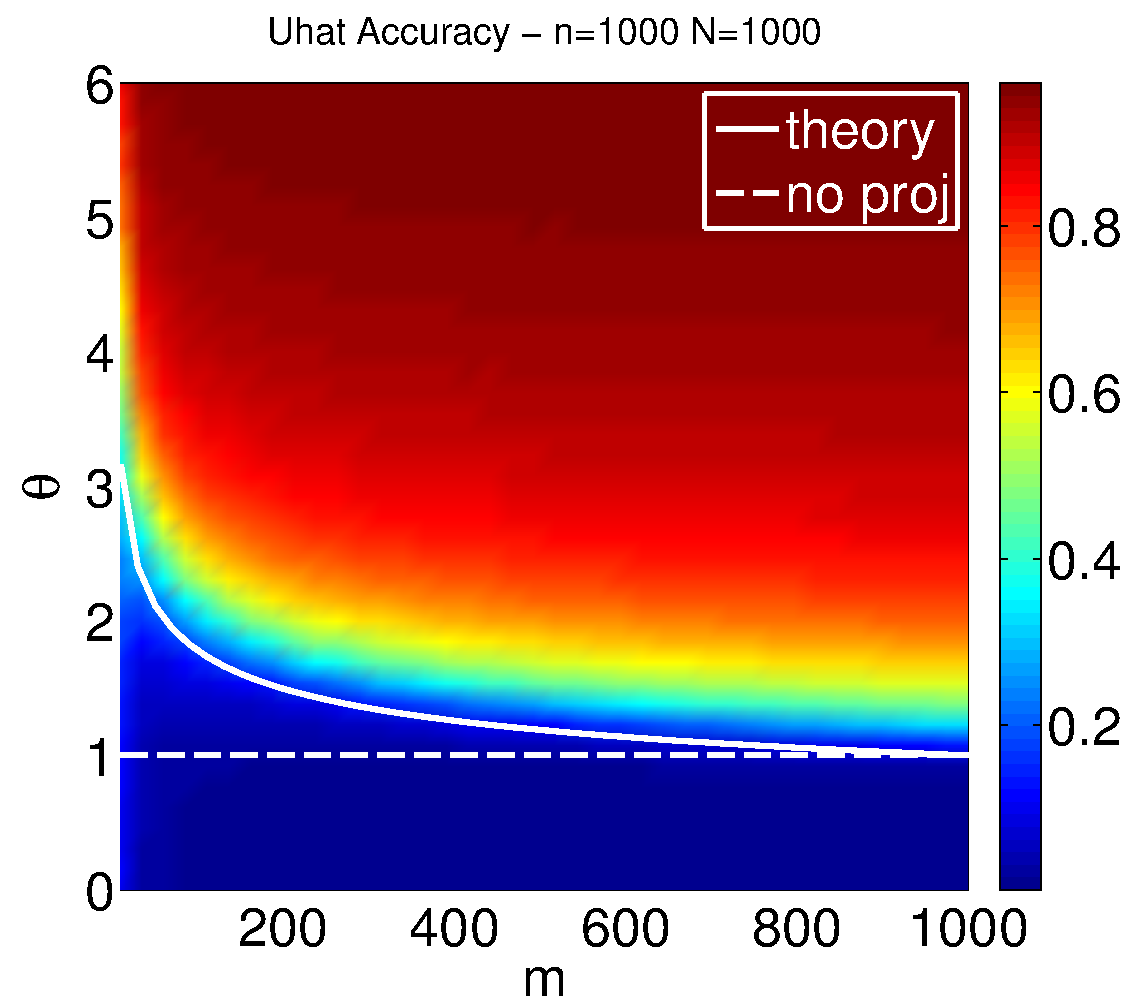
\includegraphics[width=0.357\textwidth]{chpt7_svd_proj/figs/uhat22.pdf}
%  }
  \caption{Accuracy of theoretical phase transition in Corollary
    \ref{corr:svd_proj_unitary} for unitary projection matrix $Q$ and Gaussian noise
    matrix $X$ for a rank-1 setting with fixed $n=1000$. Figure plots the KS statistic
    between singular values generated from 500 signal bearing and 500 noise only
    matrices. (a) Sweeps over both $\theta$ and $N$ for a fixed $m=100$ (b) Sweeps over
    $\theta$ and $m$ for a fixed $N=1000$.}
  \label{fig:chpt7:orth_g}
\end{center}
\end{figure}

\subsection{Comparison of Projection Matrices}

We see that the unitary projection matrix performs uniformly better than the Gaussian
projection matrix above the phase transition. Importantly, even when setting $m=n$ so that
the projection doesn't reduce the dimension, the unitary projection keeps the same phase
transition while the Gaussian projection changes the phase transition so that it is harder
to detect the presence of a signal. In terms of detection performance, the unitary
projection matrix is preferred over the Gaussian projection matrix. However, we must
consider the cost for generating these projection matrices, particularly for large
dimensions. Generating the Gaussian projection matrix is very easy as every entry is an
independent Gaussian random variable. However, generating a $n\times m$ unitary matrix for
high dimensions may be prohibitive. The analysis in this paper gives the practitioner the
ability to choose the projection matrix that best fits his or her needs. Given system
parameters, the practitioner can select the projection dimension $m$ to achieve a certain
detection ability. The decision may be driven by the ease of creating each projection
matrix.

\section{Conclusion}\label{sec:chpt7:concl}

In this paper we considered detecting low-rank multidimensional signals given multiple
noisy snapshots. Motivated by the computational cost of taking SVDs on large scale
datasets, we explored using the SVD of a projection of our data matrix to smaller
dimensional space. We analyzed the fundamental detection limits of two specific choices of
projection matrix, unitary and Gaussian. Through numerical simulations, we verified our
theoretical predictions that identified a phase transition in detection ability. Below a
critical SNR threshold, the largest singular value of the resulting projected matrix
cannot be used to infer the presence of a signal in the dataset. Importantly, we observed
that this critical threshold is lower for the unitary projection matrix than the Gaussian
projection matrix, implying that the unitary projection matrix may be used to detect
signal at lower SNRs than the Gaussian projection matrix.
